\documentclass[12pt,a4paper]{article}
\RequirePackage{etex}
\usepackage{inputenc}
\usepackage[spanish]{babel}
\usepackage{amsmath}
\usepackage{amsthm}
% \usepackage{mathtools}
\usepackage{amsfonts}
\usepackage{graphicx}
\usepackage{fourier-otf}
\usepackage{physics}
\usepackage{wrapfig}
\usepackage{multicol}
\usepackage{caption}
\usepackage{subcaption}
\usepackage{hyperref}
\usepackage[left=2cm,right=2cm,top=2cm,bottom=2cm]{geometry}
\usepackage{tikz}
\usetikzlibrary{shapes, automata, arrows}


\title{Fundamentos de redes bayesianas}
\author{Francisco J. Palmero Moya}
\date{Diciembre 2022}

\renewcommand{\labelenumi}{(\alph{enumi})}
\begin{document}
\renewcommand{\tablename}{Tabla}

\maketitle

\paragraph{Ejercicio 1.1}
Sea un grafo no dirigido $G$ que contiene cinco nodos y los siguientes enlaces: \\
$A-B$, $A-C$, $B-C$, $B-D$, $C-E$ y $D-E$.

\begin{figure}[h!]
    \centering
    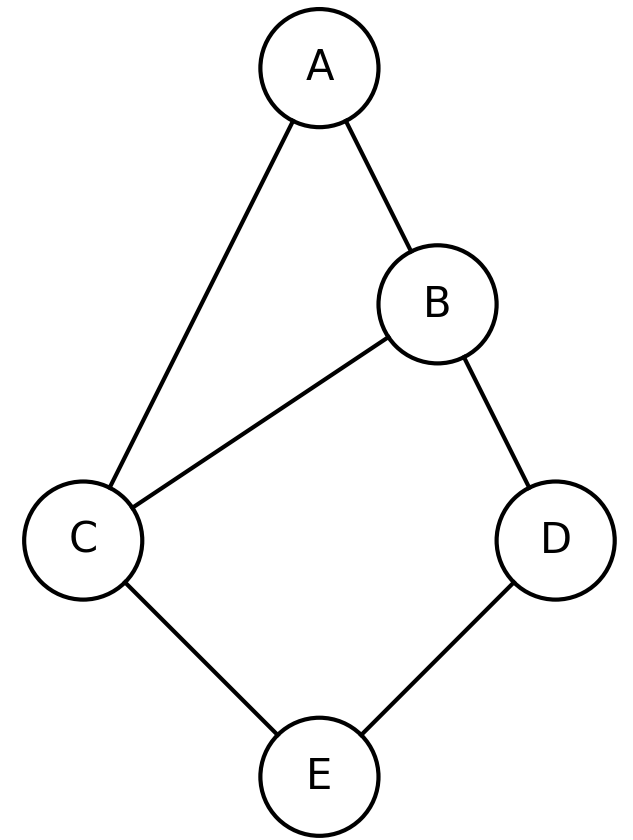
\includegraphics[width=0.25\textwidth]{graph1.png}
    \caption{Grafo no dirigido}
    \label{fig:ejercicio1}
\end{figure}

\begin{enumerate}
    \item $I_G(A, B)$: \; La relación es falsa. 
    
    Los caminos activos son:
    \begin{multicols}{2}
        \begin{itemize}
            \item $A-B$
            \item $A-C-B$
            \item $A-C-E-D-B$
        \end{itemize}
    \end{multicols}
    No hay ningún camino bloqueado.
    
    \item $I_G(B, C)$: \; La relación es falsa.
    
    Los caminos activos son:
    \begin{multicols}{2}
        \begin{itemize}
            \item $B-C$
            \item $B-A-C$
            \item $B-D-E-C$
        \end{itemize}
    \end{multicols}
    No hay ningún camino bloqueado.

    \item $I_G(A, E)$: \; La relación es falsa.
    
    Los caminos activos son:
    \begin{multicols}{2}
        \begin{itemize}
            \item $A-C-E$
            \item $A-B-C-E$
            \item $A-B-D-E$
        \end{itemize}
    \end{multicols}
    No hay ningún camino bloqueado.
    
    \item $I_G(D, E)$: \; La relación es falsa.
    
    Los caminos activos son:
    \begin{multicols}{2}
        \begin{itemize}
            \item $D-E$
            \item $D-B-C-E$
            \item $D-B-A-C-E$
        \end{itemize}
    \end{multicols}
    No hay ningún camino bloqueado.

    \item $I_G(B, C | A)$: \; La relación es falsa.
    
    Los caminos activos son:
    \begin{multicols}{2}
        \begin{itemize}
            \item $B-C$
            \item $B-D-E-C$
        \end{itemize}
    \end{multicols}
    El único camino bloqueado es:
    \begin{multicols}{2}
        \begin{itemize}
            \item $B-A-C$
        \end{itemize}
    \end{multicols}

    \item $I_G(C, D | A)$: \; La relación es falsa.
    
    Los caminos activos son:
    \begin{multicols}{2}
        \begin{itemize}
            \item $C-B-D$
            \item $C-E-D$
        \end{itemize}
    \end{multicols}
    El único camino bloqueado es:
    \begin{multicols}{2}
        \begin{itemize}
            \item $C-A-B-D$
        \end{itemize}
    \end{multicols}
    
    \item $I_G(C, D | B)$: \; La relación es falsa.
    
    El único camino activo es:
    \begin{multicols}{2}
        \begin{itemize}
            \item $C-E-D$
        \end{itemize}
    \end{multicols}
    Los caminos bloqueados son:
    \begin{multicols}{2}
        \begin{itemize}
            \item $C-B-D$
            \item $C-A-B-D$
        \end{itemize}
    \end{multicols}

    \item $I_G(C, D | A, B)$: \; La relación es falsa. Ídem al apartado (g). 
    
    Conocer $A$ no afecta a la relación entre $C$ y $D$ dado $B$.

    \item $I_G(A, E | B, C)$: \; La relación es verdadera.
    
    No hay ningún camino activo.
    Los caminos bloqueados son:
    \begin{multicols}{2}
        \begin{itemize}
            \item $A-C-E$
            \item $A-B-C-E$
            \item $A-B-D-E$
        \end{itemize}
    \end{multicols}

    \item $I_G(A, E | B, D)$: \; La relación es falsa.
    
    El único camino activo es:
    \begin{multicols}{2}
        \begin{itemize}
            \item $A-C-E$
        \end{itemize}
    \end{multicols}
    Los caminos bloqueados son:
    \begin{multicols}{2}
        \begin{itemize}
            \item $A-B-C-E$
            \item $A-B-D-E$
        \end{itemize}
    \end{multicols}
    
    \item $I_G(C, D | A, B, E)$: \; La relación es verdadera. 
    
    Todos los caminos están bloqueados:
    \begin{multicols}{2}
        \begin{itemize}
            \item $C-E-D$
            \item $C-B-D$
            \item $C-A-B-D$
        \end{itemize}
    \end{multicols}
\end{enumerate}

\newpage
\renewcommand{\labelenumi}{\arabic{enumi}.}
\renewcommand{\labelenumii}{(\alph{enumii})}
\paragraph{Ejercicio 1.2}
Sea un grafo dirigido $G$ que contiene siete nodos y los siguientes enlaces: \\
$A \to D$, $B \to D$, $B \to E$, $C \to E$, $D \to F$, $E \to F$ y $E \to G$.
\begin{figure}[h!]
    \centering
    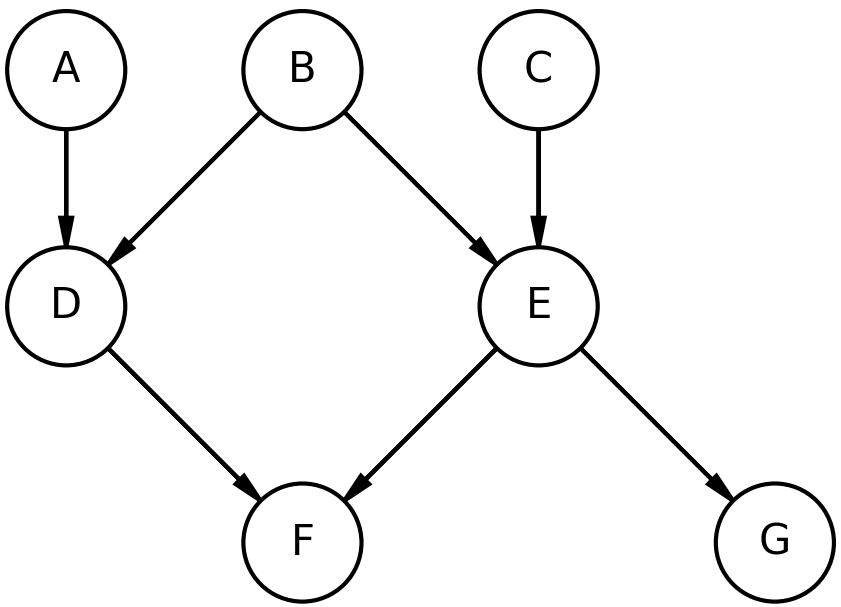
\includegraphics[width=0.4\textwidth]{graph2.png}
    \caption{Grafo dirigido}
    \label{fig:ejercicio2}
\end{figure}
\begin{enumerate}
    \item Sin condicionales.
    \begin{enumerate}
        \item $I_G(A, B)$: \; La relación es verdadera.
        
        Todos los caminos están inactivos:
        \begin{multicols}{2}
            \begin{itemize}
                \item $A \to D \leftarrow B$
                \item $A \to D \to F \leftarrow E \leftarrow B$
            \end{itemize}
        \end{multicols}

        \item $I_G(A, C)$: \; La relación es verdadera.
        
        Todos los caminos están inactivos:
        \begin{multicols}{2}
            \begin{itemize}
                \item $A \to D \leftarrow B \to E \leftarrow C$
                \item $A \to D \to F \leftarrow E \leftarrow C$
            \end{itemize}
        \end{multicols}

        \item $I_G(A, D)$: \; La relación es falsa.
        
        El único camino está activo.
        \begin{multicols}{2}
            \begin{itemize}
                \item $A \to D$
            \end{itemize}
        \end{multicols}

        \item $I_G(A, E)$: \; La relación es verdadera.
        
        Todos los caminos están inactivos:
        \begin{multicols}{2}
            \begin{itemize}
                \item $A \to D \leftarrow B \to E$
                \item $A \to D \to F \leftarrow E$
            \end{itemize}
        \end{multicols}

        \item $I_G(A, F)$: \; La relación es falsa.
        
        \begin{multicols}{2}
            El siguiente camino está activo:
            \begin{itemize}
                \item $A \to D \leftarrow F$
            \end{itemize}

            El siguiente camino está inactivo:
            \begin{itemize}
                \item $A \to D \leftarrow B \to E \to F$
            \end{itemize}
        \end{multicols}

        \item $I_G(D, E)$: \; La relación es falsa.
        
        \begin{multicols}{2}
            El siguiente camino está activo:
            \begin{itemize}
                \item $D \leftarrow B \to E$
            \end{itemize}

            El siguiente camino está inactivo:
            \begin{itemize}
                \item $D \to F \leftarrow E$
            \end{itemize}
        \end{multicols}

        \item $I_G(A, G)$: \; La relación es verdadera.
        
        Todos los caminos están inactivos:
        \begin{multicols}{2}
            \begin{itemize}
                \item $A \to D \leftarrow B \to E \to G$
                \item $A \to D \to F \leftarrow E \leftarrow G$
            \end{itemize}
        \end{multicols}

        \item $I_G(D, G)$: \; La relación es falsa.
        
        \begin{multicols}{2}
            El siguiente camino está activo:
            \begin{itemize}
                \item $D \leftarrow B \to E \to G$
            \end{itemize}

            El siguiente camino está inactivo:
            \begin{itemize}
                \item $D \to F \leftarrow E \to G$
            \end{itemize}
        \end{multicols}
        
    \end{enumerate}
    \item Añadiendo condicionales.
    \begin{enumerate}
        \item $I_G(A, B | D)$: \; La relación es falsa.
        
        \begin{multicols}{2}
            El siguiente camino está activo:
            \begin{itemize}
                \item $A \to D \leftarrow B$
            \end{itemize}

            El siguiente camino está inactivo:
            \begin{itemize}
                \item $A \to D \to F \leftarrow E \leftarrow B$
            \end{itemize}
        \end{multicols}

        \item $I_G(A, B | E)$: \; La relación es verdadera.
        
        Todos los caminos están inactivos:
        \begin{multicols}{2}
            \begin{itemize}
                \item $A \to D \leftarrow B$
                \item $A \to D \to F \leftarrow E \leftarrow B$
            \end{itemize}
        \end{multicols}

        \item $I_G(A, B | F)$: \; La relación es falsa.
        
        \begin{multicols}{2}
            El siguiente camino está activo:
            \begin{itemize}
                \item $A \to D \to F \leftarrow E \leftarrow B$
            \end{itemize}

            El siguiente camino está inactivo:
            \begin{itemize}
                \item $A \to D \leftarrow B$
            \end{itemize}
        \end{multicols}
        
        \item $I_G(A, D | B)$: \; La relación es falsa.
        
        El único camino está activo.
        \begin{multicols}{2}
            \begin{itemize}
                \item $A \to D$
            \end{itemize}
        \end{multicols}

        \item $I_G(A, E | B)$: \; La relación es verdadera.
        
        Todos los caminos están inactivos:
        \begin{multicols}{2}
            \begin{itemize}
                \item $A \to D \leftarrow B \to E$
                \item $A \to D \to F \leftarrow E$
            \end{itemize}
        \end{multicols}

        \item $I_G(C, B | G)$: \; La relación es falsa.
        
        \begin{multicols}{2}
            El siguiente camino está activo:
            \begin{itemize}
                \item $B \to E \leftarrow C$
            \end{itemize}

            El siguiente camino está inactivo:
            \begin{itemize}
                \item $B \to D \leftarrow E \leftarrow C$
            \end{itemize}
        \end{multicols}        

        \item $I_G(C, D | E)$: \; La relación es falsa.
        
        \begin{multicols}{2}
            El siguiente camino está activo:
            \begin{itemize}
                \item $D \leftarrow B \to E \leftarrow C$
            \end{itemize}

            El siguiente camino está inactivo:
            \begin{itemize}
                \item $D \to F \leftarrow E \leftarrow C$
            \end{itemize}
        \end{multicols}

        \item $I_G(A, F | D)$: \; La relación es falsa.
        
        \begin{multicols}{2}
            El siguiente camino está activo:
            \begin{itemize}
                \item $A \to D \leftarrow B \to E \to F$
            \end{itemize}

            El siguiente camino está inactivo:
            \begin{itemize}
                \item $A \to D \to F$
            \end{itemize}
        \end{multicols}    

        \item $I_G(A, F | D, E)$: \; La relación es verdadera.
        
        Todos los caminos están inactivos:
        \begin{multicols}{2}
            \begin{itemize}
                \item $A \to D \leftarrow B \to E \to F$
                \item $A \to D \to F$
            \end{itemize}
        \end{multicols}

        \item $I_G(C, F | D, E)$: \; La relación es verdadera.
        
        Todos los caminos están inactivos:
        \begin{multicols}{2}
            \begin{itemize}
                \item $C \to E \to F$
                \item $C \to E \leftarrow B \to D \to F$
            \end{itemize}
        \end{multicols}
        
        \item $I_G(A, G | B, D)$: \; La relación es verdadera.
        
        Todos los caminos están inactivos:
        \begin{multicols}{2}
            \begin{itemize}
                \item $A \to D \leftarrow B \to E \to G$
                \item $A \to D \to F \leftarrow E \to G$
            \end{itemize}
        \end{multicols}

        \item $I_G(A, G | C, D, F)$: \; La relación es verdadera.
        
        Todos los caminos están inactivos:
        \begin{multicols}{2}
            \begin{itemize}
                \item $A \to D \leftarrow B \to E \to G$
                \item $A \to D \to F \leftarrow E \to G$
            \end{itemize}
        \end{multicols}
        
    \end{enumerate}
\end{enumerate}

\newpage
\paragraph{Ejercicio 1.3}
La distribución de probabilidad $P$ viene dada por la siguiente tabla.
\begin{table}[h!]
    \centering
    \begin{tabular}{|ccc|c|}
    \hline
     $a$ & $b$ & $c$ & $P(a,b,c)$ \\
    \hline
     $+a$ & $+b$ & $+c$ & 0,12 \\
    \hline 
    $+a$ & $+b$ & $ \neg c$ & 0,03 \\
    \hline 
    $+a$ & $ \neg b$ & $+c$ & 0,48 \\
    \hline 
    $+a$ & $ \neg b$ & $ \neg c$ & 0,12 \\
    \hline
    $ \neg a$ & $+b$ & $+c$ & 0,02 \\
    \hline
    $ \neg a$ & $+b$ & $ \neg c$ & 0,08 \\
    \hline 
    $ \neg a$ & $ \neg b$ & $+c$ & 0,03 \\
    \hline
    $ \neg a$ & $ \neg b$ & $ \neg c$ & 0,12 \\
    \hline 
    \end{tabular}
    \caption{Distribución de probabilidad}
    \label{tab:my_label}
\end{table}

\begin{enumerate}
    \item Se pide comprobar la independencia, o independencia condicional, de distintas combinaciones de  las variables $A, B$ y $C$ dada la distribución de probabilidad $P$ que se muestra en la Tabla \ref{tab:my_label}.
    \begin{enumerate}
        \item $I_P(A, B)$: \; La relación es falsa.
        
        \begin{proof}
            La notación $I_P(A, B)$ representa la independencia de las variables $A$ y $B$. Las variables $A$ y $B$ son independientes si se cumple que
            \begin{align}
                P(a, b) = P(a) P(b), \hspace{0.5cm} \forall a \in A, \forall b \in B
            \end{align}\label{ec:independencia}
            Dado que las variables $A$ y $B$ son booleanas, se tiene que si 
            \begin{align*}
                P(+a, +b) = P(+a)P(+b)
            \end{align*}
            entonces la igualdad se cumple para el resto de valores\footnote{La demostración es bastante sencilla y puede encontrarse en el foro de la asignatura.}.
            
            Comenzamos calculando las probabilidades marginales $P(+a)$ y $P(+b)$.
            \begin{align*}
                P(+a) = \sum_{b \in B, c \in C} P(+a, b, c) = 0.75 \\
                P(+b) = \sum_{a \in A, c \in C} P(a, +b, c) = 0.25
            \end{align*}
            Por otro lado, tenemos:
            \begin{align*}
                P(+a, +b) = \sum_{c \in C} P(+a, +b, c) = 0.15
            \end{align*}
            Vemos que no se cumple la igualdad y por tanto $I_P(A, B)$ es falsa, esto es, las variables $A$ y $B$ están correlacionadas.
        \end{proof}

        \item $I_P(A, C)$: \; La relación es falsa.
        \item $I_P(B, C)$: \; La relación es falsa.
        \item $I_P(B, C | A)$: \; La relación es verdadera.
        
        \begin{proof}
            La notación $I_P(B, C | A)$ representa la independencia condicional de las variables $B$ y $C$ dado $A$. Las variables $B$ y $C$ son independientes dado $A$ si se cumple que
            \begin{align*}
                \forall a \in A, \forall b \in B, \forall c \in C, P(c) > 0 \Rightarrow P(b, c | a) = P(b | a) P(c | a) 
            \end{align*}
            Dada la definición de probabilidad condicionada 
            \begin{align*}
                P(x, y) = P(x | y) P(y)
            \end{align*}
            pasamos a calcular
            \begin{align*}
                \begin{cases}
                    P(+b | +a) = \frac{P(+a, +b)}{P(+a)} = 0.2 \\
                    P(\neg b | +a) = 1 - P(+b | +a) = 0.8 
                \end{cases}
                \begin{cases}
                    P(+b | \neg a) = \frac{P(\neg a, + b)}{P(\neg a)} = 0.4 \\
                    P(\neg b | \neg a) = 1 - P(+b | \neg a) = 0.6
                \end{cases}
            \end{align*}
            \begin{align*}
                \begin{cases}
                    P(+c | +a) = \frac{P(+a, +c)}{P(+a)} = 0.8 \\
                    P(\neg c | +a) = 1 - P(+c | +a) = 0.2 
                \end{cases}
                \begin{cases}
                    P(+c | \neg a) = \frac{P(\neg a, + c)}{P(\neg a)} = 0.2 \\
                    P(\neg c | \neg a) = 1 - P(+c | \neg a) = 0.8
                \end{cases}
            \end{align*}
            Finalmente vemos que por la definición de probabilidad condicionada 
            \begin{align*}
                P(x, y, z) = P(x, y | z) P(z)
            \end{align*}
            se tiene que
            \begin{align*}
                P(+b, +c | +a) & = \frac{P(+a, +b, +c)}{P(+a)} = 0.16 = P(+b | +a) P(+c | +a) \\
                P(+b, +c | \neg a) & = 0.08 = P(+b | \neg a) P(+c | \neg a) \\
                P(+b, \neg c | +a) & = 0.04 = P(+b | +a) P( \neg c | +a) \\
                P(+b, \neg c | \neg a) & = 0.32 = P(+b | \neg a) P(\neg c | \neg a) \\
                P(\neg b, +c | +a) & = 0.64 = P(\neg b | +a) P(+c | +a) \\
                P(\neg b, +c | \neg a) & = 0.12 = P(\neg b | \neg a) P(+c | \neg a)
            \end{align*}
            La igualdad se cumple para todos los valores y, por tanto, la relación es verdadera.
        \end{proof}

        \item $I_P(A, C | B)$: \; La relación es falsa.
         
        No se cumple que $P(+a, +c | +b) = P(+a | +b) P(+c | +b)$.

        \item $I_P(A, B | C)$: \; La relación es falsa.
         
        No se cumple que $P(+a, +b | +c) = P(+a | +c) P(+b | +c)$.
    \end{enumerate}
    \item Los grafos no dirigidos que son $I$-maps de $P$.
    
    Dada la definición de mapa de independencia, tenemos que una terna $(X, G, P)$ es un $I$-map de $P$ si para todo trío de subconjuntos $\left\{ A, B, C \right\}$ de $X$ (disjuntos dos a dos) se cumple que
    \begin{align}
        I_G(A, B | C) \Longrightarrow I_P(A, B | C) \equiv P(a, b | c) = P(a | c) P(b | c)
    \end{align}\label{ec:indc}
    o lo que es lo mismo
    \begin{align*}
        \neg I_P(A, B | C) \Longrightarrow \neg I_G(A, B | C)
    \end{align*}
    esto es, si las variables están correlacionadas dada la distribución de probabilidad entonces debe existir al menos un camino activo entre ambos subconjuntos del grafo.\\

    Para nuestro caso, dado que debe haber un camino activo entre 
    \begin{enumerate}
        \item[(R1)] $A$ y $B$,
        \item[(R2)] $A$ y $C$, y
        \item[(R3)] $B$ y $C$,
    \end{enumerate}
    siempre que no se apliquen condicionales,tenemos las siguientes opciones

    \begin{figure}[h!]
        \centering
        \begin{subfigure}{0.3\textwidth}
            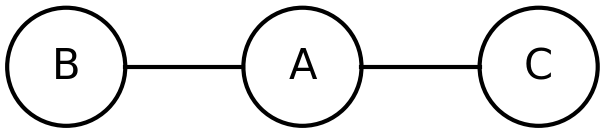
\includegraphics[width=\textwidth]{graph321.png}
            \caption{Opción A}
            \label{fig:graph321}
        \end{subfigure}
        \hfill
        \begin{subfigure}{0.3\textwidth}
            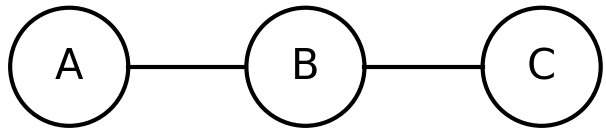
\includegraphics[width=\textwidth]{graph322.png}
            \caption{Opción B}
            \label{fig:graph322}
        \end{subfigure}
        \hfill
        \begin{subfigure}{0.3\textwidth}
            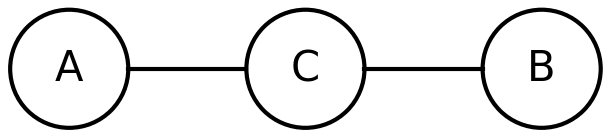
\includegraphics[width=\textwidth]{graph323.png}
            \caption{Opción C}
            \label{fig:graph323}
        \end{subfigure}
        \hfill
        \begin{subfigure}{0.3\textwidth}
            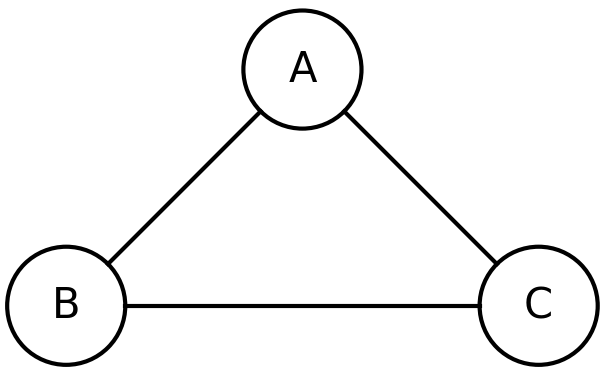
\includegraphics[width=\textwidth]{graph324.png}
            \caption{Opción cíclica}
            \label{fig:graph324}
        \end{subfigure}
        \caption{Posibles soluciones sin condicionales}
    \end{figure}
    Sin embargo, vemos que no se cumple las siguientes condiciones 
    \begin{align*}
        \text{Opción B:} \hspace{1cm} \neg I_P(A, C | B) \Longrightarrow \neg I_G(A, C | B) \\
        \text{Opción C:} \hspace{1cm} \neg I_P(A, B | C) \Longrightarrow \neg I_G(A, B | C)
    \end{align*}
    no se cumplen y, por tanto, no pueden ser $I$-maps de $P$. 

    Finalmente, cabe resaltar que la Opción cíclica no refleja la independencia condicional entre las variables $B$ y $C$ dado $A$. Aunque esto no influye en su condición de $I$-map, ya que no tiene porqué representarla (véase \eqref{ec:indc}).
    \subparagraph*{Solución} 
    Los únicos $I$-maps son: Grafo (\ref{sub@fig:graph321}) y Grafo (\ref{sub@fig:graph324}).

    \item Los grafos dirigidos acíclicos que son $I$-maps de $P$.
    
    Análogamente al apartado anterior, tenemos que encontrar grafos que cumplan las relaciones entre las variables de forma que existan caminos activos cuando las variables estén relacionadas. No se incluye el procedimiento por simplicidad.

    \subparagraph*{Solución}
    Las siguientes GDAs son $I$-maps de $P$

    \begin{figure}[h!]
        \centering
        \begin{subfigure}{0.3\textwidth}
            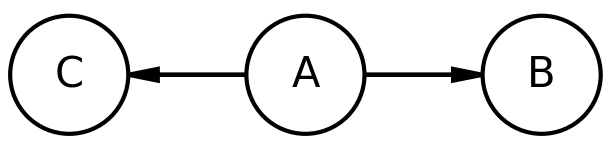
\includegraphics[width=\textwidth]{graph331.png}
            \caption{Head-to-head}
            \label{fig:graph331}
        \end{subfigure}
        \hfill
        \begin{subfigure}{0.3\textwidth}
            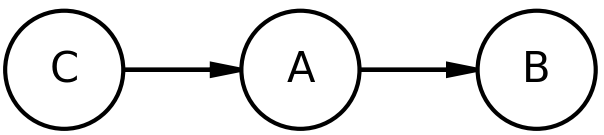
\includegraphics[width=\textwidth]{graph332.png}
            \caption{Tail-to-head}
            \label{fig:graph332}
        \end{subfigure}
        \hfill
        \begin{subfigure}{0.3\textwidth}
            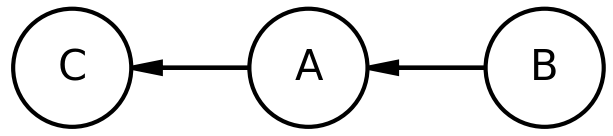
\includegraphics[width=\textwidth]{graph333.png}
            \caption{Tail-to-head}
            \label{fig:graph333}
        \end{subfigure}
        \caption{Grafos dirigidos acíclicos que son $I$-maps de $P$}
    \end{figure}
\end{enumerate}

\newpage
\paragraph{Ejercicio 1.4}
\begin{enumerate}
    \item Red bayesiana del problema.
    
    \begin{figure}[h!]
        \centering
        \begin{tikzpicture}[main/.style = {draw, ellipse}] 
            \node[main] at (0, 5) (T) {Enfermedad T};
            \node[main] at (0, 3) (A) {Enfermedad A};
            \node[main] at (3, 1) (S) {Síntoma S};
            \node[main] at (5, 4) (B) {Enfermedad B};
            \node[main] at (7, 1) (L) {Laboratorio L};

            \draw [-to] (T) -- (A);
            \draw [-to] (A) -- (S);
            \draw [-to] (B) -- (S);
            \draw [-to] (B) -- (L);
            \end{tikzpicture} 
        \caption{Red bayesiana}
    \end{figure}

    \item Valores de cada variable.
    \begin{itemize}
        \item Enfermedad T ($T$): Padecida ($+t$) / No padecida ($-t$)
        \item Enfermedad A ($A$): Presente ($+a$) / Ausente ($-a$)
        \item Síntoma S ($S$): Presente ($+s$) / Ausente ($-s$)
        \item Enfermedad B ($B$): Presente ($+b$) / Ausente ($-b$)
        \item Laboratorio L ($L$): Positiva ($+l$) / Negativa ($-l$)
    \end{itemize}
\end{enumerate}

\end{document}
